% Build from the repository root with:
% latex -output-directory=figures figures/Figure1.tex
% dvips -o figures/Figure1.ps figures/Figure1.dvi
% ps2epsi figures/Figure1.ps figures/Figure1.eps
\documentclass{minimal}
\usepackage{tikz}
\usetikzlibrary{arrows.meta,intersections,positioning}

\begin{document}
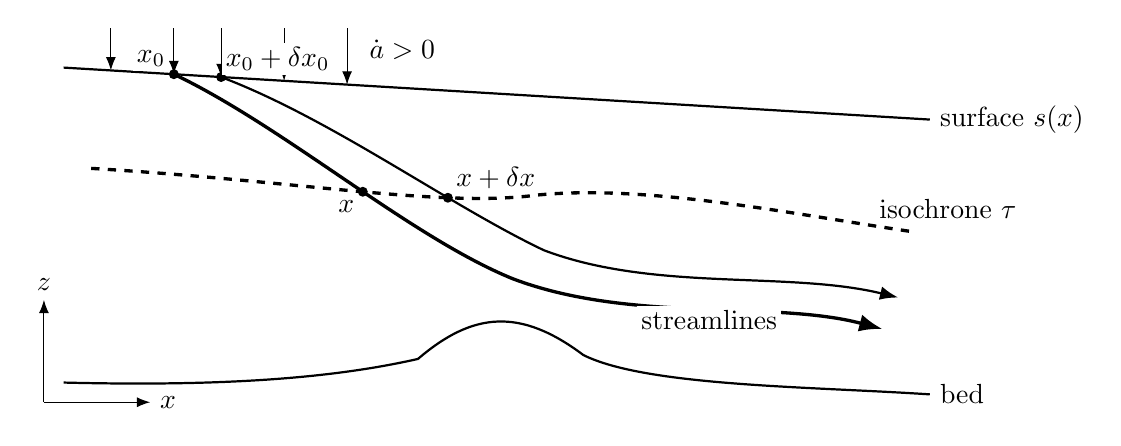
\begin{tikzpicture}[x=1cm,y=1cm,>=Latex,labelbox/.style={fill=white,inner sep=1.5pt}]
  % domain
  \draw[thick] (0,4.5) -- (11,3.84) node[right] {surface $s(x)$};
  \draw[thick] (0,0.5) .. controls (2,0.45) and (3.4,0.55) .. (4.5,0.8)
    .. controls (5.2,1.4) and (5.8,1.45) .. (6.6,0.85)
    .. controls (7.4,0.45) and (9.5,0.45) .. (11,0.35) node[right] {bed};
  % accumulation arrows
  \foreach \x in {0.6,1.4,2.0,2.8,3.6} {
    \pgfmathsetmacro{\ys}{4.5-0.06*\x}
    \draw[->] (\x,5.0) -- (\x,\ys);
  }
  \node[labelbox] at (4.3,4.72) {$\dot a>0$};
  % neighboring trajectories, each beginning at the accumulation surface
  \draw[name path=streamline0,->,very thick]
    (1.4,4.416) .. controls (2.8,3.75) and (4.4,2.35) .. (5.7,1.82)
    .. controls (7.2,1.25) and (9.0,1.55) .. (10.4,1.18);
  \draw[name path=streamline1,->,thick]
    (2.0,4.38) .. controls (3.4,3.85) and (4.9,2.75) .. (6.1,2.18)
    .. controls (7.5,1.65) and (9.2,1.92) .. (10.6,1.58);
  \node[labelbox] at (8.2,1.3) {streamlines};
  % an equal-age surface intersecting both trajectories once
  \draw[name path=agecurve,dashed,very thick]
    (0.35,3.22) .. controls (3.0,3.06) and (4.8,2.72) .. (6.0,2.88)
    .. controls (7.4,3.02) and (9.2,2.65) .. (10.75,2.42);
  \node[labelbox,right] at (10.3,2.7) {isochrone $\tau$};
  % deposition and equal-age positions
  \fill (1.4,4.416) circle (1.8pt);
  \fill (2.0,4.38) circle (1.8pt);
  \node[labelbox,above left] at (1.35,4.45) {$x_0$};
  \node[labelbox,above right] at (2.0,4.4) {$x_0+\delta x_0$};
  \path[name intersections={of=streamline0 and agecurve,by=p0}];
  \path[name intersections={of=streamline1 and agecurve,by=p1}];
  \fill (p0) circle (1.8pt) node[labelbox,below left=2pt] {$x$};
  \fill (p1) circle (1.8pt) node[labelbox,above right=2pt] {$x+\delta x$};
  % axes
  \draw[->] (-0.25,0.25) -- (1.1,0.25) node[right] {$x$};
  \draw[->] (-0.25,0.25) -- (-0.25,1.55) node[above] {$z$};
\end{tikzpicture}
\end{document}
